\section{Boilers }\label{boilers}

\subsection{Simple Hot Water Boiler}\label{simple-hot-water-boiler}

The input object Boiler:HotWater provides a simple model for boilers that only requires the user to supply the nominal boiler capacity and thermal efficiency. An efficiency curve can also be used to more accurately represent the performance of non-electric boilers but is not considered a required input. The fuel type is input by the user for energy accounting purposes.

The model is based the following three equations

\begin{equation}
OperatingPartLoadRatio = \frac{{BoilerLoad}}{{BoilerNomCapacity}}
\end{equation}

\begin{equation}
TheoreticalFuelUse = \frac{{BoilerLoad}}{{NominalThermalEfficiency}}
\end{equation}

\begin{equation}
FuelUsed = \frac{{TheoreticalFuelUse}}{{BoilerEfficiencyCurveOuput}}
\end{equation}

-or-

\begin{equation}
FuelUsed = \frac{{BoilerLoad}}{{\left( {NominalThermalEfficiency} \right)\left( {BoilerEfficiencyCurveOutput} \right)}}
\end{equation}

The final equation above includes the impact of the optional boiler efficiency performance curve. To highlight the use of the normalized boiler efficiency curve, the fuel use equation is also shown in an expanded format. The normalized boiler efficiency curve represents the changes in the boiler's nominal thermal efficiency due to loading and changes in operating temperature. If the optional boiler efficiency curve is not used, the boiler's nominal thermal efficiency remains constant throughout the simulation (i.e., BoilerEfficiencyCurveOutput = 1).

When a boiler efficiency performance curve is used, any valid curve object with 1 or 2 independent variables may be used. The performance curves are accessed through EnergyPlus' built-in performance curve equation manager (curve objects). The linear, quadratic, and cubic curve types may be used when boiler efficiency is solely a function of boiler loading, or part-load ratio (PLR). These curve types are used when the boiler operates at the specified setpoint temperature throughout the simulation. Other curve types may be used when the boiler efficiency can be represented by both PLR and boiler operating temperature. Examples of valid single and dual independent variable equations are shown below. For all curve types, PLR is always the x independent variable. When using curve types with 2 independent variables, the boiler water temperature (Twater) is always the y independent variable and can represent either the inlet or outlet temperature depending on user input.

\subsubsection{Single independent variable:}\label{single-independent-variable}

\begin{itemize}
\item
  \(BoilerEfficiencyCurve = C1 + C2\left( {PLR} \right)\) ~(Linear)
\item
  \(BoilerEfficiencyCurve = C1 + C2\left( {PLR} \right) + C3{\left( {PLR} \right)^2}\) (Quadratic)
\item
  \(BoilerEfficiencyCurve = C1 + C2\left( {PLR} \right) + C3{\left( {PLR} \right)^2} + C4{(PLR)^3}\) (Cubic)
\end{itemize}

\subsubsection{Dual independent variables:}\label{dual-independent-variables}

\begin{itemize}
\item
  \(BoilerEfficiencyCurve = C1 + C2\left( {PLR} \right) + C3{\left( {PLR} \right)^2} + \left( {C4 + C5\left( {PLR} \right) + C6{{\left( {PLR} \right)}^2}} \right)\left( {Twater} \right)\) (QuadraticLinear)
\item
  \(BoilerEfficiencyCurve = C1 + C2\left( {PLR} \right) + C3{\left( {PLR} \right)^2} + C4\left( {Twater} \right) + C5{(Twater)^2} + C6(PLR)(Twater)\) ~(Biquadratic)
\item
  \(BoilerEfficiencyCurve = C1 + C2\left( {PLR} \right) + C3{\left( {PLR} \right)^2} + C4\left( {Twater} \right) + C5{(Twater)^2} + C6\left( {PLR} \right)\left( {Twater} \right) + C7{(PLR)^3} + C8{(Twater)^3} + C9{\left( {PLR} \right)^2}\left( {Twater} \right) + C10\left( {PLR} \right){(Twater)^2}\) (Bicubic)
\end{itemize}

When a boiler efficiency curve is used, a constant efficiency boiler may be specified by setting C1 = 1 and all other coefficients to 0. A boiler with an efficiency proportional to part-load ratio or which has a non-linear relationship of efficiency with part-load ratio will typically set the coefficients of a linear, quadratic, or cubic curve to non-zero values. Using other curve types allows a more accurate simulation when boiler efficiency varies as a function of part-load ratio and as the boiler outlet water temperature changes over time due to loading or as changes occur in the water temperature setpoint.

The parasitic electric power is calculated based on the user-defined parasitic electric load and the operating part load ratio calculated above. The model assumes that this parasitic power does not contribute to heating the water.

\begin{equation}
{P_{parasitic}} = {P_{load}}\left( {PLR} \right)
\end{equation}

where:

\({P_{parasitic}}\) = parasitic electric power (W), average for the simulation time step

\({P_{load}}\) ~~~ = parasitic electric load specified by the user (W)

\subsection{Steam Boiler}\label{steam-boiler}

\subsubsection{Description of Model}\label{description-of-model}

A steam boiler is the essential part of a building steam heating system and can be described as primary driver of the steam loop.~ It is the component that maintains the desired loop temperature.

The emphasis in EnergyPlus was laid on developing a building simulation model for steam boiler with ability to model detailed boiler performance without the cost of exhaustive user inputs to the boiler model.~ The Boiler:Steam input object is used on the plant loop supply side of EnergyPlus with the primary purpose of supplying steam to the heating coils, which constitute the demand side of the loop.

The steam boiler is a variable mass flow rate device.~ The mass flow rate of steam through the boiler is determined by the heating demand on the loop which in turn is determined by the equipment that is hooked to the demand side of the loop, namely the steam coils and hot water heater.~ In short, the steam coil determines the mass flow rate of steam required for heating the zone to its required setpoint, the mixer sums up the total steam demanded by each of the individual coils and reports it to the boiler via the pump.

\begin{figure}[hbtp] % fig 158
\centering
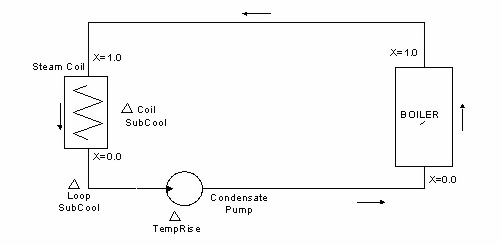
\includegraphics[width=0.9\textwidth, height=0.9\textheight, keepaspectratio=true]{media/image2932.png}
\caption{Schematic of Steam Boiler in the Steam loop \protect \label{fig:schematic-of-steam-boiler-in-the-steam-loop}}
\end{figure}

Figure~\ref{fig:schematic-of-steam-boiler-in-the-steam-loop} describes the rudimentary loop structure with steam flowing from coils to boiler.~ It is essential to mention that it is the coils that determine the mass of steam required and the boiler simply delivers the required mass flow at desired temperature provided it is adequately sized.~ The algorithm for determining the mass flow rate is structured on the demand side and the variable flow boiler has no role to play in determining the steam mass flow.

Figure~\ref{fig:schematic-of-steam-boiler-operation} outlines the simple steam boiler model.~ Sub cooled water enters the variable flow boiler through the pump, the boiler inputs energy to water stream consuming fuel, boiler losses are accounted via boiler efficiency.~ The boiler delivers steam at a quality equal to 1.0 at saturated condition.

The advantage of steam heating systems over hot water is the high latent heat carrying capacity of steam, which reduces the mass flow rate of the fluid required.~ The amount of superheated and sub cooled heat transfer in Steam heating systems is negligible, latent heat transfer accounts for almost all of the heat exchange into the zones via steam to air heat exchangers.

\begin{figure}[hbtp] % fig 159
\centering
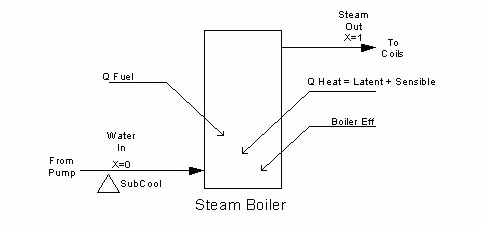
\includegraphics[width=0.9\textwidth, height=0.9\textheight, keepaspectratio=true]{media/image2933.png}
\caption{Schematic of Steam Boiler Operation \protect \label{fig:schematic-of-steam-boiler-operation}}
\end{figure}

Boiler Load is a summation of sensible and latent heat addition to the water stream as described with the following equation.~ The mass flow rate through the boiler is known, while delta temp is the temperature difference between the boiler inlet and boiler outlet.~ Latent heat of steam is calculated at loop operating temperature.

\begin{equation}
{Q_B} = \,\dot m\, \times \left[ {({c_{p,w}} \times \Delta T)\,\,\, + \,\,\,{h_{fg}}} \right]
\end{equation}

Theoretical fuel used is calculated with the following equation.~ Boiler efficiency is a user input and accounts for all the losses in the steam boiler.

\begin{equation}
{F_t} = \frac{{{Q_B}}}{{{\eta_B}}}
\end{equation}

The operation part load ratio is calculated with the following equation.~ This is later used to calculate the actual fuel consumption, its ratio of boiler load to boiler nominal capacity.

\begin{equation}
{O_{PLR}} = \frac{{{Q_B}}}{{{Q_{B,N}}}}
\end{equation}

The actual fuel consumption by the boiler is calculated as using the following equation, where C1, C2, and C3 are the Part Load Ratio coefficients.

\begin{equation}
{F_{}} = \frac{{{F_t}}}{{{C_1}\,\, + \,\,{C_2}\,\, \times \,\,{O_{PLR}}\,\, + \,\,{C_3} \times \,{O_{PLR}}^2\,}}
\end{equation}

Essentially the boiler model provides a first order approximation of performance for fuel oil, gas, and electric boilers.~ Boiler performance is based on theoretical boiler efficiency and a single quadratic fuel use-part load ratio curve represented in the equation above.~ This single curve accounts for all combustion inefficiencies and stack losses.

The control algorithm for a steam boiler is an important issue.~ The user may want the boiler to be undersized and in such a case it will not be able to meet the demand side steam flow request.~ Subsequently the boiler load exceeds the boiler nominal capacity.~ The boiler operates at its nominal capacity but is unable to meet the plant heating demand.~ Pseudo code from EnergyPlus has been used to describe the control logic used in the steam boiler simulation.

*********************PSEUDO CODE SECTION STARTS***********************

At start of simulation an initial value of steam mass flow rate is calculated.~ This is required to start the flow of steam around the loop.

\begin{equation}
If\,\,\,\,(FirstTimeThrough)\,\,\,THEN
\end{equation}

Calculate the boiler supply steam mass flow rate at start of simulation.

\begin{equation}
\,{\dot m_s}\,\, = \,\,\frac{{{Q_B}}}{{{h_{fg\,\,\, + }}\,\,{c_{p,w}}\,\, \times \Delta {T_{loop}}\,\,}}
\end{equation}

\(ELSE\) ~~ ! Not first time through

Steam boiler calculations rely heavily on the variable \(\dot m\) \(_{b}\), boiler mass flow rate.~ This variable \(\dot m\) \(_{b}\) is the assigned equal to mass flow at boiler inlet node for preliminary calculations.

\begin{equation}
\,{\dot m_b}\,\,\, = \,\,\,\mathop {\,{{\dot m}_{Inlet_Node}}}\limits^{}
\end{equation}

Calculating the boiler delta temperature difference between the inlet and outlet nodes.~ This calculation is used to determine various boiler control situation.

\begin{equation}
\Delta {T_{in_out}}\,\, = \,\,{T_{SP}}\,\, - \,\,{T_{in}}
\end{equation}

In case the temperature difference calculated with the previous equation equation~ is zero then the boiler just needs to supply latent heat to steam, else the boiler performs its normal load calculations by providing both sensible and latent heat to the inlet stream.

\begin{equation}
If\,\,(\Delta {T_{in_out}}\,\, < \,\,\,\,0\,\,\,)\,\,\,THEN
\end{equation}

\begin{equation}
{Q_B}\,\, = \,\,\,{\dot m_b}\,\,\, \times \,\,{h_{fg}}
\end{equation}

\begin{equation}
ELSE
\end{equation}

\begin{equation}
{Q_B}\,\, = \,\,\,{\dot m_b}\,\,\, \times \,\,(\,\,\,{h_{fg}} + \,\,{c_{p,w}} \times \Delta {T_{in_out}}\,\,)
\end{equation}

\begin{equation}
End\,\,If
\end{equation}

Sometimes the boiler load Q\(_{B}\) is greater than the demand side requested load at the current time step, which may occur because the boiler inlet conditions is from previous time step.~ There is sudden fall in request of steam mass flow from the demand side.~ The boiler now recalculates its new mass flow and adjusts to these new conditions.

\begin{equation}
If\,\,({Q_B}\,\, > \,\,{Q_{HeatingDemand}}\,\,\,)\,\,\,THEN
\end{equation}

Boiler load is set equal to the new boiler heating demand and steam mass flow rate is recalculated.

\begin{equation}
{Q_B}\,\, = \,\,{Q_{HeatingDemand}}
\end{equation}

\begin{equation}
\,{\dot m_s}\,\,\, = \,\,\frac{{{Q_B}}}{{{h_{fg\,\,\, + }}\,\,{c_{p,w}}\,\, \times \Delta {T_{loop}}\,\,}}
\end{equation}

\begin{equation}
End\,\,If
\end{equation}

In case the requested load exceeds the boiler nominal capacity, which is its maximum heating capacity.~ In this case the requested steam mass flow is not met and the zone is not heated adequately.~ This happens if the boiler is undersized.~ The steam mass flow rate is recalculated at nominal capacity.

\begin{equation}
If\,\,({Q_B}\,\, > \,\,{Q_{No\min al_Capacity}}\,\,\,)\,\,\,THEN
\end{equation}

Boiler load is set equal to boiler nominal capacity and steam mass flow rate recalculated.

\begin{equation}
{Q_B}\,\, = \,\,{Q_{No\min al_Capacity}}
\end{equation}

\begin{equation}
\,{\dot m_s}\,\,\, = \,\,\frac{{{Q_B}}}{{{h_{fg\,\,\, + }}\,\,{c_{p,w}}\,\, \times \Delta {T_{loop}}\,\,}}
\end{equation}

\begin{equation}
End\,\,If
\end{equation}

\begin{equation}
End\,\,If
\end{equation}

End If statement for the boiler load control algorithm.~ This algorithm determines all possible control conditions that might while simulating a system in EnergyPlus.

*********************PSEUDO CODE SECTION STARTS***********************

If the boiler operating pressure exceeds the maximum allowable boiler pressure, the simulation trips and outputs a warning regarding the same.~ This notifies the user about potential system pressure sizing problems.

Integration of the steam boiler simulation model in EnergyPlus required developing number of subroutines, which operate in sequence.~ These subroutines are designed to read inputs from the input file, initialize the variables used in the boiler simulation model, simulate the boiler performance, update the node connections, and report the required variables.~ In case the user has difficulty with boiler inputs, provisions have been made to auto size the boiler nominal capacity and maximum steam flow rate.~ These two values play an important role in sizing the boiler.

\subsubsection{Model Assumptions}\label{model-assumptions}

The EnergyPlus boiler model is ``simple'' in the sense that it requires the user to supply the theoretical boiler efficiency.~ The combustion process is not considered in the model.~ The model is independent of the fuel type, which is input by the user for energy accounting purposes only.~ This is an ideal model for Building Simulation Program such that it utilizes the desired amount of resources in terms of simulation run time, but successfully provides fairly good sizing parameters for an actual boiler.

It is assumed that the steam boiler operates to maintain a desired temperature, the temperature being saturation temperature of steam and corresponding to this saturation temperature there exist a single value of saturation pressure at which the loop operates.~ Hence the boiler could either be saturation pressure controlled or temperature controlled.~ Since users would have better idea of steam temperatures rather than pressure the boiler inputs are designed for temperature control.

\subsubsection{Nomenclature for Steam Loop}\label{nomenclature-for-steam-loop}

% table 50
\begin{longtable}[c]{p{1.0in}p{4.0in}}
\caption{Steam Loop Nomenclature \label{table:steam-loop-nomenclature}} \tabularnewline
\toprule 
\({Q_{B}}\) & Boiler Heat Transfer. W. \tabularnewline
\midrule
\endfirsthead

\caption[]{Steam Loop Nomenclature} \tabularnewline
\toprule 
\({Q_{B}}\) & Boiler Heat Transfer. W. \tabularnewline
\midrule
\endhead

\({Q_{B,N}}\) & Boiler Nominal Capacity.~ W. \tabularnewline
\({O_{PLR}}\) & Boiler Operating Part Load Ratio.~ \tabularnewline
\(\Delta\)T\(_{sc}\) & Degree of subcooling in coil.~ \tabularnewline
\(\Delta\)T\(_{in_out}\) & Temperature difference across the steam boiler.~ ºC. \tabularnewline
\(\rho\)\(_{w}\) & Density of condensate entering the pump.~ Kg/m\(^3\).~ \tabularnewline
\(Q_{Des}\) & Design Load on the steam coil.~ W. \tabularnewline
\(h_{f,n}\) & Enthalpy of fluid at point n on the Ts diagram.~ J/kg. \tabularnewline
\(P_{Frac}\) & Fraction of Pump Full Load Power.~ W. \tabularnewline
\(F_{m,f}\) & Fractional Motor Power Lost to Fluid.~ W. \tabularnewline
\(Q_{a,l}\) & Heating load on the Air Loop Steam Coil.~ W. \tabularnewline
\(Q_{z,c}\) & Heating load on the Zone Steam Coil.~ W. \tabularnewline
\(h_{fg,T_loop}\) & Latent heat of steam at Loop operating Temperature.~ J/kg. \tabularnewline
\(h_{fg}\) & Latent Heat of Steam.~ J/kg. \tabularnewline
\(Q_{L,H}\) & Latent Heat Part of the Heating Coil Load.~ W. \tabularnewline
\(\Delta\)Q\(_{loss}\) & Loop losses in steam coil.~ W. \tabularnewline
\(\Delta\)T\(_{loop}\) & Loop Temperature Difference. \tabularnewline
\(\dot m_{a}\) & Mass flow rate for steam coil Kg/s. \tabularnewline
\(\dot m_{in}\) & Mass flow rate of steam entering the steam coil .Kg/s. \tabularnewline
\(\dot m_{a,l}\) & Mass flow rate of steam for Air loop steam coil Kg/s \tabularnewline
\(\dot m_{z,c}\) & Mass flow rate of steam for zone steam coil Kg/s. \tabularnewline
\(\dot m_{s}\) & Mass flow rate of steam.~ Kg/s. \tabularnewline
\(\dot m_{loop}\) & Mass flow rate of steam for the steam loop.~ Kg/s. \tabularnewline
\(\dot m\) & Mass of condensate entering the pump.~ Kg/s. \tabularnewline
\(\dot m_{a,max}\) & Maximum allowed mass flow rate of air.~ Kg/s \tabularnewline
\(\dot m_{S,max}\) & Maximum Mass flow rate of steam Kg/s \tabularnewline
\(\dot m_{B,Supply}\) & Maximum steam mass flow rate supplied by boiler.~ Kg/s. \tabularnewline
\(\dot V_{w,max}\) & Maximum Volume flow rate of condensate in pump.~ m\(^3\)/s. \tabularnewline
\(\dot V_{w,loop}\) & Maximum Volume flow rate of condensate in steam loop.~ m\(^3\)/s. \tabularnewline
\(T_{a,in,min}\) & Minimum inlet air temperature possible.~ ºC. \tabularnewline
\(P_{n}\) & Nominal Power Capacity for condensate pump.~ W. \tabularnewline
\(P_{nom}\) & Nominal power of the pump.~ W. \tabularnewline
\(H_{n}\) & Nominal Pump Head.~ M. \tabularnewline
\(\dot V_{nom}\) & Nominal volume flow rate through the condensate pump.~ m\(^3\)/s. \tabularnewline
PLR & Part Load Ratio for condensate pump. \tabularnewline
\(\eta\)\(_{p}\) & Pump efficiency. \tabularnewline
\(\eta\)\(_{m}\) & Pump Motor Efficiency. \tabularnewline
P & Pump Power.~ W. \tabularnewline
\(Q_{S,H}\) & Sensible Heat Part of the Heating Coil Load.~ W. \tabularnewline
\(T_{sp}\) & Setpoint Temperature of the zone.~ ºC. \tabularnewline
\(T_{a,out,SP}\) & Setpoint air outlet temperature for the steam coil.~ ºC. \tabularnewline
\(P_{S}\) & Shaft power of the pump.~ W. \tabularnewline
\(c_{p,a}\) & Specific Heat Capacity for Air.~ J/Kg K. \tabularnewline
\(c_{p,w}\) & Specific Heat Capacity for Water.~ J/Kg K. \tabularnewline
\(\eta\)\(_{B}\) & Steam Boiler Efficiency. \tabularnewline
\(T_{a,in}\) & Temperature of air entering the coil.~ ºC. \tabularnewline
\(T_{a}\) & Temperature of air entering the steam coil.~ ºC. \tabularnewline
\(T_{a,out}\) & Temperature of air leaving the coil.~ ºC. \tabularnewline
\(T_{s,in}\) & Temperature of steam entering the coil.~ ºC. \tabularnewline
\(F_{in}\) & Theoretical Fuel Consumption by the Steam Boiler.~ W. \tabularnewline
\(\dot m_{coils,R}\) & Total Mass flow rate requested by all the steam coils.~ Kg/s. \tabularnewline
\(\dot V\) & Volume of condensate entering the pump.~ m\(^3\)/s. \tabularnewline
\(T_{w,out}\) & Water outlet temperature from pump.~ ºC. \tabularnewline
\bottomrule
\end{longtable}

\subsubsection{References}\label{references-007}

ASHRAE Handbook. 1996. HVAC Systems and Equipment, Air Conditioning and Heating Systems.~ Chapter 10, Steam Systems.~ pp.\emph{~} 10.1-10.16. 1996.

\emph{BLAST 3.0 Users Manual}. 1999. Building Systems Laboratory.~ Urbana-Champaign: Building Systems Laboratory, Department of Mechanical and Industrial Engineering, University of Illinois.

Chillar, R.J. 2005. ``Development and Implementation of a Steam Loop In The Building Energy Simulation Program EnergyPlus,'' M.S. Thesis, Department of Mechanical and Industrial Engineering, University of Illinois at Urbana-Champaign.

\emph{TRNSYS 16 User Manual}. 2004. A Transient System Simulation Program. Solar Energy Laboratory, Madison. University of Wisconsin-Madison.

El-Wakil, M. M. 1984. Power Plant Technology, McGraw Hill, New York, pp.~~ 30-72.

Babcock \& Wilcox. 1978. Steam-Its Generation and Use, The Babcock \& Wilcox Company, New York ,Section I, II, IV, and VII.

S.A. Klein. 2004. Engineering Equation Solver EES. University of Wisconsin Madison.
